% Complete 12-page working manuscript; generated by scripts/build-length-variants.mjs.
% ACM working format; target-venue compliance requires the conference handoff.
% !TeX program = pdflatex
\documentclass[sigconf,nonacm]{acmart}

\usepackage{graphicx}
\usepackage{xurl}

\setcopyright{none}
\settopmatter{printacmref=false,authorsperrow=2}
\renewcommand\footnotetextcopyrightpermission[1]{}
\renewcommand{\textbullet}{\textnormal{-}}
\renewcommand{\labelitemi}{\textnormal{-}}
\emergencystretch=2em

\newif\ifarchsyncanonymous
\ifdefined\archsyncanonymousmode
  \archsyncanonymoustrue
\else
  \archsyncanonymousfalse
\fi
\newcommand{\archsyncrepository}[2]{%
  \ifarchsyncanonymous
    \nolinkurl{#1} (blinded)%
  \else
    \href{#2}{\nolinkurl{#1}}%
  \fi
}
\newcommand{\archsynccommit}[4]{%
  \ifarchsyncanonymous
    \texttt{#1} commit \texttt{#4} (blinded artifact)%
  \else
    \href{#2/commit/#3}{\texttt{#1} commit \texttt{#4}}%
  \fi
}

\begin{document}

\title{ArchSync: Evidence-Backed Detection of Architecture Drift in TypeScript Systems}

\author{Vo Duc Hieu}
\orcid{0009-0007-5389-5177}
\authornote{Corresponding author.}
\affiliation{%
  \department{Software Engineering}
  \institution{FPT University}
  \city{Ho Chi Minh City}
  \country{Vietnam}
}
\email{voduchieu@littleboys.biz}

\author{Tran Minh Hoang}
\orcid{0009-0000-0302-1841}
\affiliation{%
  \department{Computer Science and Engineering}
  \institution{VNUK Institute for Research and Executive Education, The University of Danang}
  \city{Da Nang}
  \country{Vietnam}
}
\email{an1dee@littleboys.biz}

\author{Ha Hoang Bach}
\orcid{0009-0000-5118-0660}
\affiliation{%
  \department{Information Assurance}
  \institution{FPT University}
  \city{Ho Chi Minh City}
  \country{Vietnam}
}
\email{bachcp6@littleboys.biz}

\author{Le Van Kiet}
\orcid{0009-0007-8434-882X}
\affiliation{%
  \department{Software Engineering}
  \institution{VNUK Institute for Research and Executive Education, The University of Danang}
  \city{Da Nang}
  \country{Vietnam}
}
\email{levankiet1212.2004@littleboys.biz}

\begin{abstract}
Software teams can keep builds green while implementation relationships drift away from an approved architecture, leaving reviewers without a repeatable way to decide whether a change is harmless, forbidden, or a legitimate evolution. This paper presents ArchSync, a deterministic architecture-conformance prototype that treats a machine-readable model as an executable contract and reconstructs an observed service graph from TypeScript source code. Stack-specific analyzers detect selected HTTP, PostgreSQL, Redis, and AMQP interactions, preserve file-level evidence, and feed a Git-diff gate that maps introduced findings to PASS, BLOCK, or REVIEW without rewriting the approved model. We verify the prototype on two co-developed development datasets and replay the same controlled changes through the incremental gate. Within these finite regression sets, the implementation agrees with the declared graph, decision, evidence-location, and full-scan oracles, and provenance tracking removes the targeted detector errors exposed by the earlier analyzer. An external-tool comparison remains proposed and was not executed within the reported evaluation; no accepted comparator result or common label mapping is available, and the study lacks an independently curated real-world holdout. Its results therefore establish executable-contract coherence and reproducible regression behavior only, not comparative advantage or general accuracy on TypeScript systems.
\end{abstract}


\begin{CCSXML}
<ccs2012>
 <concept>
  <concept_id>10011007.10010940.10010941.10010942</concept_id>
  <concept_desc>Software and its engineering~Software architectures</concept_desc>
  <concept_significance>500</concept_significance>
 </concept>
 <concept>
  <concept_id>10011007.10011074.10011099</concept_id>
  <concept_desc>Software and its engineering~Software verification and validation</concept_desc>
  <concept_significance>300</concept_significance>
 </concept>
</ccs2012>
\end{CCSXML}

\ccsdesc[500]{Software and its engineering~Software architectures}
\ccsdesc[300]{Software and its engineering~Software verification and validation}

\keywords{software architecture, architecture conformance, architecture drift, static analysis, architecture as code, software evolution}

\maketitle

\section{Introduction}

Software architecture captures the intended decomposition of a system, the responsibilities of its components, and the relationships that are permitted between them. As systems evolve, this intent can diverge from implementation; recent mapping and developer studies report structural violations, effects on maintenance and evolution, and continuing reliance on documentation and shared practices \cite{li2022erosion,anthony2024drifting}. A locally reasonable change can bypass a gateway, couple an interface directly to a database, or introduce infrastructure without an explicit architecture decision while compilation and functional tests continue to pass.

For teams whose architecture intent is not connected to executable checks, documentation alone leaves a gap between intended and implemented structure. ArchSync addresses this workflow problem with a deterministic, evidence-backed connection between architecture intent and implementation. A diagram can communicate the desired system but is difficult to use as an automated quality gate. Conversely, a source-derived dependency graph can expose implementation relationships but does not by itself state which relationships are allowed, forbidden, required, or merely require review.

We present ArchSync, an architecture-conformance workflow based on two graphs. The expected graph is derived from a versioned \texttt{architecture.yaml} document containing components, relationships, and deterministic rules. The observed graph is inferred from source code by stack-specific analyzers. ArchSync compares the graphs and produces one of three classifications: \emph{no-impact} when implementation conforms without topology changes, \emph{violation} when one or more rules are broken, and \emph{evolution} when a non-forbidden topology change requires human review. Findings retain both the model location that establishes the expectation and the source location supporting the observation.

For pull requests, the workflow compares findings at the Git merge base with findings at the proposed head. Only findings introduced by the change determine its gate decision: violations block, non-forbidden topology changes request review, and changes without new drift pass. The observed graph therefore follows implementation changes, while the expected graph remains the approved design baseline. Our proposed governance workflow requires an explicit model change and architecture-owner review to accept evolution; the evaluated command reports the need for review but does not manage approval or rejection records.

The prototype deliberately focuses on TypeScript and Node.js. It recognizes HTTP calls through \texttt{fetch}, PostgreSQL access through \texttt{pg}, Redis operations, and AMQP publishing and consumption. This is an empirical boundary rather than a claim that architecture drift is TypeScript-specific: the expected graph, rule engine, finding contract, and metrics are language-neutral, while each additional language requires a separately implemented and evaluated source-to-graph analyzer. The bounded TypeScript scope permits deterministic contracts and reproducible measurement without probabilistic inference. Large-language-model explanations and automatic repairs are excluded from the decision path.

This paper makes the following contributions:
\begin{itemize}
  \item a machine-readable architecture contract with typed components and relationships plus deny, allow, require, and require-path rules;
  \item a provenance-aware TypeScript source-to-graph pipeline with file, line, column, detector, snippet, and confidence evidence;
  \item a three-way decision model separating violations from topology evolution;
  \item a Git-diff gate with cached baseline graphs, component-incremental analysis, GitHub annotations, and explicit handling of introduced, pre-existing, and resolved findings;
  \item a reproducible 20-patch controlled development benchmark plus a 40-signal positive/hard-negative regression corpus, with explicit evidence boundaries.
\end{itemize}

\section{Background and Related Work}

This section is a scoped narrative synthesis selected to establish context for ArchSync's design, not a systematic literature review. Sources were drawn from the retained keyword-search corpus and selected for their relevance to architecture conformance, drift detection, and static-analysis reliability, with emphasis on 2022--2025 publications. Four earlier works are retained as concept-origin references. Selection was purposive rather than exhaustive; the discussion distinguishes evaluated techniques, tool demonstrations, and secondary syntheses, and does not establish the absence of competing approaches.

\subsection{Architecture Erosion and Reconstruction}

Architecture erosion denotes progressive misalignment between intended architecture and implementation. A mapping study of 73 primary studies characterizes its manifestations and consequences \cite{li2022erosion}. Evidence from two OpenStack projects identifies erosion symptoms in code reviews \cite{li2022symptoms}; a subsequent journal study examines violation symptoms and developer responses across OpenStack and Qt projects \cite{li2023warnings}. These related studies offer concrete developer-facing evidence, but their overlapping project contexts should not be counted as independent replications. A mixed-methods study further identifies documentation, clear responsibilities, and shared practices as ways developers manage drift \cite{anthony2024drifting}. Together, these findings motivate implementation-linked checks without reducing architecture quality to one structural metric.

Reconstruction recovers architectural views from implementation artifacts. Ducasse and Pollet's foundational taxonomy distinguishes bottom-up, top-down, and hybrid processes \cite{ducasse2009reconstruction}. A recent tertiary mapping organizes the applicability of recovery approaches, emphasizing that selecting an appropriate method depends on its context and assumptions \cite{sar2024taxonomy}. A microservice-focused mapping compares the purposes, inputs, and outputs of reconstruction tools and identifies availability and maintenance concerns \cite{bakhtin2024mapping}. These syntheses provide context for method selection rather than a uniform benchmark of tool accuracy. View-based drift analysis demonstrates how reconstructed specifications can be compared with intended models in an industrial case study \cite{uzun2024drift}. ArchSync adopts a narrower observation boundary: an explicit expected model and a defined set of service and infrastructure relationships.

\subsection{Static Architecture Conformance}

Software Reflexion Models compare a high-level model with a source-derived model and distinguish convergence, divergence, and absence \cite{murphy1995reflexion}. Knodel and Popescu compare several static conformance formulations \cite{knodel2007comparison}, while Dependency Constraint Language expresses allowed and forbidden dependencies in object-oriented systems \cite{terra2009dcl}. These works supply the conceptual origins of expected-versus-observed comparison and dependency rules; neither concept is claimed as new here.

Recent tools adapt conformance checking to particular languages and deployment settings. CALint checks Python implementations against the Clean Architecture dependency rule and accompanies detection with refactoring support \cite{calint2022}. ArchLintor is a particularly close language-level comparison: it detects architectural violations in TypeScript systems, reports module relationships, and supports CI/CD integration \cite{archlintor2025}. ArchSync focuses on typed service-topology observations and a versioned finding contract, whereas this ArchLintor description centers on module-interaction checking. No head-to-head comparison with ArchLintor is reported.

IaC coupling-conformance metrics extend architecture checking to deployment practices \cite{ntentos2022iac}, providing a relevant reference for ArchSync's planned, unevaluated IaC extension. In a correction-oriented approach, 3Erefactor searches for executable refactorings that reduce architectural inconsistency \cite{refactor2024}; ArchSync currently reports findings and gate outcomes rather than generating repairs. Language Models as Architectural Gatekeepers explores converting natural-language design rules into executable conformance tests \cite{lucena2025gatekeepers}. Its preliminary evaluation distinguishes tests that execute from tests that correctly express the intended rule. ArchSync instead evaluates explicit rules deterministically. This design avoids dependence on generated rules at decision time, but determinism alone does not establish detector accuracy or superiority over an LLM-assisted approach.

The prototype combines typed HTTP, data, and asynchronous edges; explicit require and require-path semantics; source and model evidence in a versioned finding contract; and separate violation and evolution outcomes. This is an implementation-specific positioning within the reviewed work, not an exhaustive novelty claim.

\subsection{Change-Time Conformance}

Architectural change can be examined at several time scales. Commit-level prediction relates source changes to architectural changes \cite{commits2025}; a predicted change is not necessarily a violation of intended architecture. Repository mining combined with static reconstruction tracks microservice architectural evolution across development history \cite{evolution2024}. View-based drift analysis compares recovered and intended specifications \cite{uzun2024drift}, while an industrial conformance-visualization study reports practitioner feedback and challenges involving scalability, usability, and workflow integration \cite{thermofisher2025}. These approaches motivate change-aware feedback but evaluate different questions and should not be treated as interchangeable baselines.

ArchSync places its comparison at pull-request time and exposes deterministic findings through annotations and exit-code decisions. Its current evidence verifies change-scoped behavior on a co-developed benchmark. It does not establish industrial adoption, reduced developer effort, organizational effectiveness, or comparative performance against the reviewed tools.

\subsection{Evaluation and Static-Analysis Reliability}

Konersmann et al. examine evaluation and replication support in software-architecture research \cite{konersmann2022replicability}. Abgaz et al.'s review concerns monolith-to-microservice decomposition \cite{abgaz2023decomposition}; that adjacent scope should not be treated as a direct measurement of architecture-conformance accuracy or proof that suitable conformance baselines do not exist. A more direct precedent is Schneider et al.'s comparison of static microservice-recovery tools: it identifies 13 tools, executes nine, and reports both individual and combined-tool recovery performance \cite{schneider2025comparison}. This provides a concrete model for future external-baseline work. ArchSync has not reproduced that benchmark, and its typed-edge detector results cannot be compared numerically without aligning capabilities and ground truth.

Static-analysis-based visual models expose microservice dependencies at a system level \cite{staticmodels2024}. Recovery from multiple dependency models explores how complementary relations affect reconstructed structure \cite{dependencies2024}. These approaches motivate the future multi-source direction discussed for ArchSync, while leaving its current evidence restricted to the declared TypeScript source patterns. Secondary mappings and tertiary taxonomies help organize this space; they are not additional independent trials of each underlying tool.

False positives and false negatives remain central to reliability. Interrogation testing distinguishes precision and soundness issues and demonstrates failures in mature analyzers \cite{kaindlstorfer2024interrogation}. ArchSync consequently includes annotated positive and hard-negative signals alongside topology changes. Its manifests, pinned artifacts, explicit denominators, and replay checks support reproducibility, but do not turn the synthetic development benchmark into representative evidence. The narrative synthesis establishes design context and comparison dimensions; it supports neither coverage-completeness claims nor absence-of-evidence claims.

\section{Problem Definition}

Let the expected architecture contract be
\begin{equation}
  M = (C_E, E_E, R),
\end{equation}
where $C_E$ is the set of expected components, $E_E$ is the set of expected typed and directed relationships, and $R$ is the set of conformance rules. We denote the graph projection of this contract by $G_E=(C_E,E_E)$. A relationship is represented as a tuple $(u,t,v)$, where $u$ is the source component, $v$ is the target component, and $t$ is the relationship type.

Given a source-code repository $S$, a stack-specific analyzer $A$ constructs an observed graph
\begin{equation}
  G_O = A(S) = (C_O, E_O, P),
\end{equation}
where $C_O$ and $E_O$ are observed components and relationships, and $P$ maps each observation to source evidence. Source evidence contains a repository-relative file path, line, column, detector identifier, excerpt, and a fixed detector confidence annotation; the latter is not a calibrated correctness probability.

ArchSync supports four deterministic rule semantics. A \emph{deny} rule rejects every matching relationship. An \emph{allow} rule constrains the outgoing relationships of selected sources to an allowed target set. A \emph{require} rule states that every matching source must have a direct edge to a matching target. A \emph{require-path} rule states that every matching source must reach a matching target through a non-empty directed path. Rules may optionally constrain the relationship type and may use wildcard component selectors.

The conformance function compares $M$ and $G_O$ and returns a graph difference $\Delta$, a set of rule violations $\mathcal{V}$, and a set of evidence-backed findings $\mathcal{F}$. Its classification is defined as
\begin{equation}
\operatorname{class}(M,G_O)=
\begin{cases}
\text{violation}, & \text{if } |\mathcal{V}| > 0,\\
\text{evolution}, & \text{if } |\mathcal{V}| = 0 \land |\Delta| > 0,\\
\text{no-impact}, & \text{otherwise.}
\end{cases}
\end{equation}

For a Git change from base repository $S_b$ to head repository $S_h$, ArchSync computes base and head finding sets and compares them by stable semantic identity:
\begin{equation}
  \mathcal{F}^{+} = \mathcal{F}(M,A(S_h)) \setminus \mathcal{F}(M,A(S_b)).
\end{equation}
Only $\mathcal{F}^{+}$ controls the pull-request decision. A newly introduced rule finding yields BLOCK; introduced evolution findings yield REVIEW; an empty $\mathcal{F}^{+}$ yields PASS. Findings in both sets are pre-existing, while findings only at the base are resolved. This distinction prevents an unrelated change from being blocked by historical drift without allowing new drift to enter silently.

The research problem is to determine whether a source analyzer can reconstruct enough architectural information to make this classification accurately, reproducibly, and with actionable evidence. A useful solution must minimize both missed architectural relationships and spurious relationships, preserve stable outputs for identical inputs, and separate rule-breaking changes from topology changes that may be valid but require approval.

\section{Research Questions}

\textbf{RQ1: How accurately can ArchSync reconstruct software architecture components and relationships from TypeScript source code?}

For the 20-patch development benchmark (D1), this question reports matched, extra, and missed graph elements and patch deltas. For the separate 40-signal corpus (D2), it reports descriptive precision, recall, F1, true negatives, and specificity against the annotated detector signals; these are controlled-corpus results, not population estimates.

\textbf{RQ2: How accurately can ArchSync distinguish no-impact changes, architecture-rule violations, and architecture evolution?}

This question evaluates exact classification agreement with a manually curated ground truth and, for violations, agreement on the expected rule identifiers.

\textbf{RQ3: How accurately can ArchSync localize architectural findings in source code?}

This question evaluates whether a finding identifies the expected changed file and exact source line. Column, detector, excerpt, and model path are retained as additional diagnostic evidence.

\textbf{RQ4: Are ArchSync full-repository and Git-diff outputs deterministic and reproducible, and what analysis scope and latency are observed for the cached incremental gate?}

This question compares normalized observed graphs, findings, and pull-request decisions across repeated executions and clean installations. For Git-diff checks it additionally records cache behavior, files parsed relative to the head repository, and cold/warm latency on the measured environment.

\section{Proposed Approach}

\subsection{Architecture as an Executable Contract}

ArchSync uses a YAML document as the source of truth for architecture intent. The model defines stable component identifiers, component types, layers, directed relationships, rule severity, ownership metadata, and optional quality goals. JSON Schema validation rejects malformed documents, while semantic validation rejects unknown component references, duplicate edges, invalid identifiers, and other topology inconsistencies. Mermaid and draw.io views are derived from the model; they are not independent sources of truth.

The validated model is converted into an expected graph with stable node identifiers and canonical edge keys. This normalization makes graph comparison and evidence manifests reproducible. It also enables the same conformance semantics to be used by command-line tools, benchmark evaluation, and continuous-integration adapters.

\subsection{Source-to-Graph Analysis}

A Guardian analyzer traverses TypeScript files under component roots and parses them through the TypeScript Compiler API. Rather than matching arbitrary text, detectors inspect syntax-tree nodes, imports, call expressions, variable initialization, environment-variable references, and URL literals. Stack-specific detectors translate these signals into typed architectural relationships.

The detector set recognizes HTTP requests, PostgreSQL clients and queries, Redis clients and operations, and AMQP publishing and consumption. Version 0.2 tracks local bindings introduced by named, aliased, and namespace imports from \texttt{pg}, \texttt{redis}, and \texttt{amqplib}. PostgreSQL and Redis edges require an operation on an identifier associated with a recognized client initializer; AMQP edges require a channel associated with a tracked connection. These associations use per-file identifier names rather than complete compiler symbol or alias resolution. This package provenance filters same-named methods on unrelated objects when their receivers lack a tracked association; it does not establish soundness under arbitrary shadowing or reassignment. Endpoint resolution uses explicit literals and deterministic environment-variable fallbacks when available. Every detected relationship carries one or more source locations. Detected components and relationships are sorted and deduplicated before serialization.

\subsection{Conformance and Decision Semantics}

The conformance engine first computes node and edge differences between the expected and observed graphs. It then evaluates the observed graph against the architecture rules. A rule violation takes precedence over ordinary topology evolution. This is a fixed conservative policy: one rule violation determines the top-level classification even when the change also contains acceptable evolution. Both types of findings remain available for inspection. Rule severity is reported but does not alter this precedence or the blocking threshold. This avoids reducing a forbidden edge to a reviewable addition, while potentially delaying otherwise acceptable changes bundled with it; alternative severity- or context-dependent policies are not evaluated.

The repository-facing decision is derived from the classification:
\begin{itemize}
  \item \textbf{PASS} for no-impact changes;
  \item \textbf{BLOCK} for deterministic rule violations; and
  \item \textbf{REVIEW} for non-forbidden architecture evolution.
\end{itemize}
The REVIEW outcome separates a request for a design decision from a detected rule breach. In the evaluated command, PASS, BLOCK, and REVIEW return exit codes 0, 1, and 3, respectively. A repository must configure its merge controls to treat the nonzero REVIEW result as requiring resolution; an annotation alone does not enforce approval. ArchSync reports the change without automatically modifying the approved architecture contract.

\subsection{Diff-Scoped Living Architecture Loop}

The Phase 3 gate resolves the merge base, enumerates modified, added, deleted, renamed, and untracked files, and maps changed TypeScript paths to source components. A cold check reconstructs the base Observed Graph from the committed source tree. The graph is cached inside Git metadata under a key derived from the base commit, architecture-contract hash, and analyzer version. A warm check validates and reuses that cache.

For the proposed head, Guardian parses all TypeScript files in affected source components, rather than only changed lines, so independently detectable relationships elsewhere in those components are retained. This wider scan scope does not provide inter-file client or data-flow resolution. Evidence and relationships owned by those components replace their baseline counterparts; unaffected components remain from the cached graph. Base and head are then evaluated with the same Core semantics, and stable finding identities determine introduced, pre-existing, and resolved findings. GitHub workflow commands annotate source locations, a Markdown artifact summarizes the graph delta, and exit codes implement the merge gate.

This mechanism updates observations without authorizing design changes. The expected model remains versioned in Git and is never rewritten by the analyzer. The proposed governance workflow accepts evolution through an explicit model change reviewed by architecture owners. The evaluated gate does not authenticate that approval or persist accepted/rejected review decisions. If a reviewer rejects an evolution and the code and contract remain unchanged, rerunning the gate returns REVIEW again, not BLOCK. The team must reject the merge through repository controls, revise or remove the implementation change, and rerun the check. Recording the rationale and introducing a reviewed rule when the rejection expresses a lasting constraint are proposed governance actions, not automatic rejection handling implemented by this experiment.

\subsection{Evidence-Rich Findings}

A finding contains a stable contract version, identifier, kind, severity, message, optional rule identifier, affected component or edge, source evidence, and model evidence. For an observed forbidden edge, the evidence points to the call site that introduced the relationship. For a missing required edge or path, the source component is used as a deterministic anchor and the relevant rule location is retained as model evidence.

This separation allows the deterministic engine to state \emph{what} changed and \emph{why} it violates the contract, while preserving enough context for a developer or architect to inspect the implementation.

\section{System Architecture}

Figure~\ref{fig:architecture} separates approved intent from base and proposed implementation state. ArchSync Core validates the model and provides the expected graph and executable rules. Guardian caches a base Observed Graph, scopes the Git diff to affected source components, incrementally constructs the head graph, and preserves source evidence. The gate compares base and head findings before deriving the pull-request decision.

\begin{figure*}[t]
  \centering
  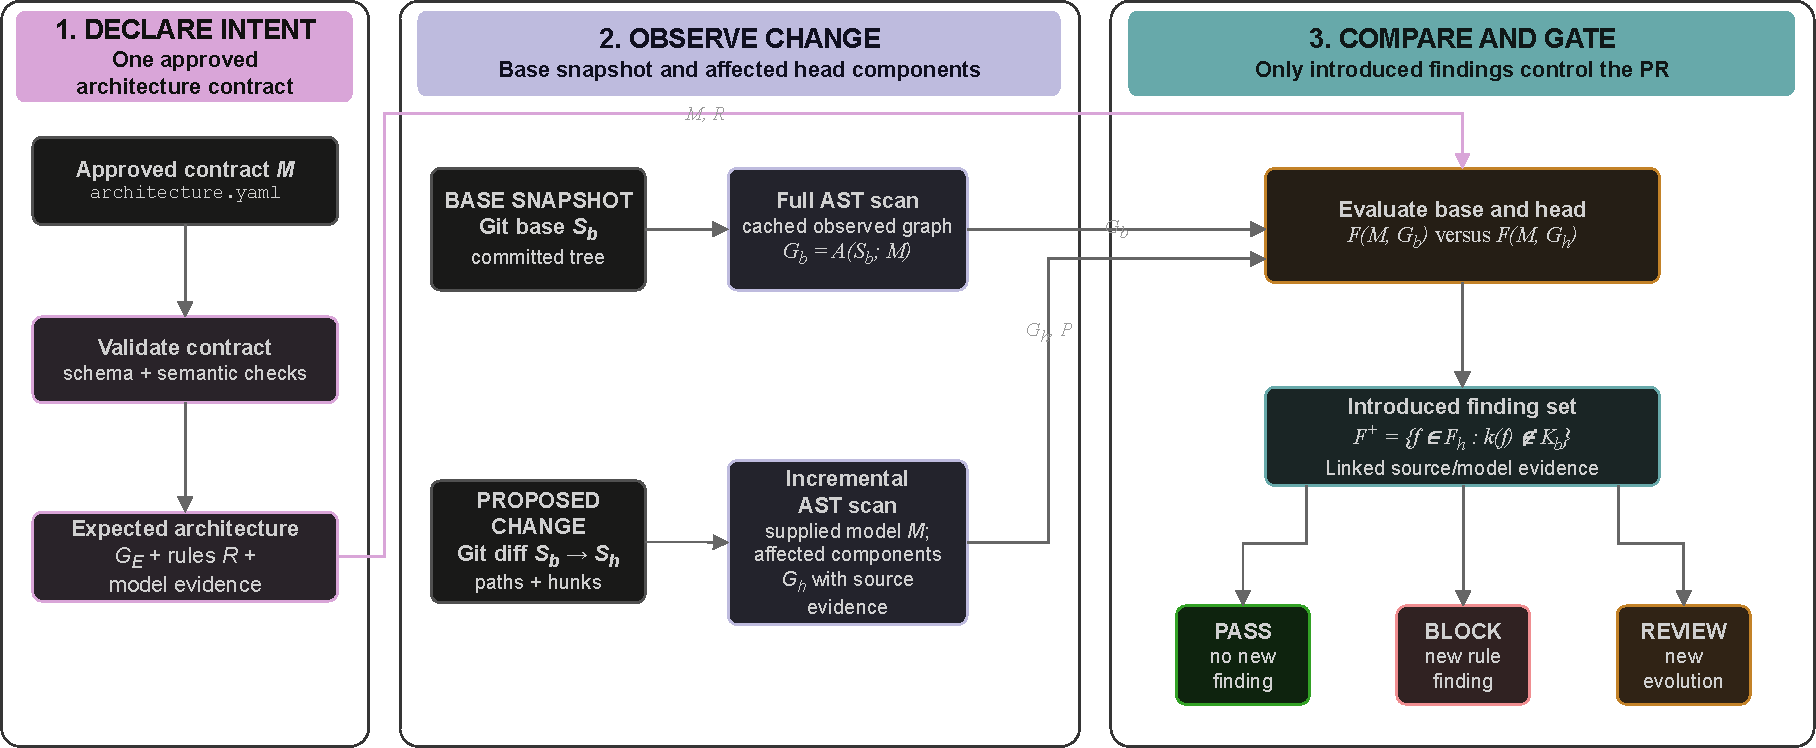
\includegraphics[width=\textwidth]{figures/Fig-1.pdf}
  \caption{ArchSync Phase 3 system architecture. The three-stage pipeline separates approved intent, base/head observation, and the pull-request gate. The model remains authoritative; only findings introduced by the Git diff determine PASS, BLOCK, or REVIEW.}
  \Description{Stage one validates the approved architecture contract into an expected graph, rules, and model evidence. Stage two builds a cached base graph and incrementally reconstructs the proposed head with source evidence. Stage three compares base and head findings, keeps the introduced set, and maps it to PASS, BLOCK, or REVIEW.}
  \label{fig:architecture}
\end{figure*}

The architecture is divided across focused repositories. \archsyncrepository{archsync-core}{https://github.com/Little-Boy-s-ArchSync/archsync-core} contains the architecture contract and deterministic conformance functions. \archsyncrepository{archsync-guardian}{https://github.com/Little-Boy-s-ArchSync/archsync-guardian} contains analyzers and findings. \archsyncrepository{archsync-benchmark}{https://github.com/Little-Boy-s-ArchSync/archsync-benchmark} contains the controlled development benchmark. \archsyncrepository{archsync-examples}{https://github.com/Little-Boy-s-ArchSync/archsync-examples} contains readable models and generated views. \archsyncrepository{archsync-mcp}{https://github.com/Little-Boy-s-ArchSync/archsync-mcp} is reserved for a later interaction layer and is excluded from the initial experiment. The named draft exposes these real repository links; the double-blind build replaces them with blinded artifact labels.

\section{Implementation}

\subsection{Prototype and Detector Logic}

\archsyncrepository{archsync-core}{https://github.com/Little-Boy-s-ArchSync/archsync-core} implements the architecture contract, schema and semantic validation, normalized graph comparison, and deny/allow/require/require-path rules. \archsyncrepository{archsync-guardian}{https://github.com/Little-Boy-s-ArchSync/archsync-guardian} implements TypeScript extraction, source evidence, and the Git-diff gate. Guardian delegates conformance semantics to Core so repository and incremental checks use the same rule engine.

For a concrete PostgreSQL example, consider the following code inside the \texttt{order-service} component:
\begin{verbatim}
import { Pool as PgPool } from "pg";
const db = new PgPool({
  connectionString: "postgres://postgres:5432/orders"
});
await db.query("select 1");
\end{verbatim}
The import detector records \texttt{PgPool} as a local name for a recognized \texttt{pg} constructor. The initializer pass recognizes \texttt{new PgPool}, resolves the inline \texttt{connectionString}, and associates \texttt{db} with target \texttt{postgres}, derived from the URL hostname. At \texttt{db.query}, the call detector requires that receiver association before emitting the directed edge $(\texttt{order-service},\texttt{data},\texttt{postgres})$. Merely importing \texttt{pg}, constructing an unrelated client, or calling an unrelated object's \texttt{query} method does not satisfy this detector. Construction alone does not emit the database-access edge. Evidence identifies the query call's file, line, column, detector, and excerpt.

The analysis uses per-file identifier maps and four passes over variable declarations; it is not general alias analysis or interprocedural data-flow analysis. Imported client wrappers, arbitrary reassignment, shadowed identifiers, and relationships requiring resolution across files are not comprehensively handled. Endpoint resolution uses literals, mapped variables, and naming conventions such as \texttt{DATABASE\_URL} for \texttt{postgres}. For binary expressions it tries the right-hand expression first; this deterministic heuristic does not evaluate runtime environment values or branch conditions. The PostgreSQL evidence confidence of 0.99 is a fixed detector annotation, not a calibrated probability. Redis operations similarly require a recognized client, and AMQP operations require a channel associated with a recognized connection.

\subsection{Controlled Evaluation Artifact}

\archsyncrepository{archsync-benchmark}{https://github.com/Little-Boy-s-ArchSync/archsync-benchmark} supplies the synthetic Order Platform, 20 executable patches with group-authored ground truth, and the 40-signal positive/hard-negative corpus. Each patch runs on a fresh copy. Git-diff experiments additionally construct a baseline commit, perform cold and warm checks, and compare incremental head observations with a separate full scan. This full scan checks incremental equivalence; it does not independently establish extraction accuracy.

The reported measurements use pinned Core and Guardian revisions, preserved source and patch manifests, and raw result artifacts. Verification checks artifact integrity and recomputes derived results. Revision identifiers, package hashes, coverage and smoke-test counts, historical verification commands, and the code-level detector/gate audit are supplied in the supplementary implementation audit. These controls make the experiment inspectable; they are not a research contribution or evidence of accuracy on external systems. \texttt{archsync-mcp} is not used in the experiment.

\section{Controlled Verification Methodology}

\subsection{Experimental Objects}

The evaluation uses two controlled TypeScript/Node.js datasets. Dataset D1 is an end-to-end Order Platform benchmark whose expected baseline contains five components and five directed relationships. Twenty patches are distributed as nine no-impact changes, seven rule violations, and four architecture evolutions. In addition to refactoring, service bypass, required-edge removal, Redis, and AMQP cases from the initial benchmark, the expansion includes documentation-only URLs, type-only imports, method-name lookalikes, direct gateway database access, allow-rule violations, a broken multi-hop path, aliased PostgreSQL construction, a new service, and a Redis hash operation.

Each D1 case declares changed files, expected graph delta, classification, findings, and source location. The topology labels and classifications originated in Phase 1. Patch implementations and exact evidence lines were refined while the Phase 2 analyzer was integrated. D1 is therefore a development benchmark and regression oracle, not a blinded holdout. Validators check structural consistency, distribution, patch applicability, changed-file membership, patch-hunk containment, and integrity hashes; they do not replace independent semantic review.

Dataset D2 is a detector challenge corpus with five groups: \texttt{fetch}, PostgreSQL, Redis, AMQP publish, and AMQP consume. Each group contains four positive and four hard-negative source lines, giving 20 positives and 20 negatives. Positive variants include aliases, namespace imports, environment fallbacks, and multiple supported operations. Hard negatives include URL text without a call, custom functions, unused package imports, local objects with detector-shaped method names, lifecycle calls, comments, and string literals. The manifest binds each signal to a detector, source file, exact line, expected edge, description, and required source substring.

D2 was authored after the initial v0.1 analyzer and deliberately targets its weaknesses. We execute both the frozen v0.1 artifact and provenance-aware v0.2 on the same corpus. This paired comparison identifies concrete regression behavior but is not an unbiased estimate of improvement on unseen programs.

The Phase 3 protocol reuses D1 rather than introducing a third dataset. For each case, it creates a fresh Git repository from the unchanged baseline, commits that baseline with fixed author metadata, applies one patch to the working tree, and runs the diff gate twice. The first execution reconstructs and caches the base graph; the second must hit the cache. A separate full scan of the same patched head acts as an equivalence oracle for the incremental result. Ground truth is extended operationally with expected changed files and the PASS/BLOCK/REVIEW mapping already implied by each D1 label. We compare normalized cold and warm results, decisions, changed-file sets, exact architecture deltas, rule identifiers, evidence locations, and incremental/full-scan equivalence. Timings are retained only from the recorded Windows run because shared CI runners do not provide a controlled performance environment.

Figure~\ref{fig:evaluation-protocol} summarizes the executable verification protocol and shows how raw analyzer executions become the reported metrics and evidence artifact.

\subsection{External-Comparison Boundary}

External comparison remains future work; it was not executed within the reported evaluation. No accepted comparator result or common label mapping is available. A module-dependency analyzer is a candidate because it can express constraints on static dependencies in JavaScript/TypeScript, but selecting a tool does not establish equivalence between its observations and ArchSync's typed service relationships. That equivalence must be defined and reviewed before comparative measurements are interpreted.

The proposed comparison must distinguish the unit being labeled, the relationship a detector can observe, and the architecture rule applied to that relationship. A module import and a remote service call may occur in the same file without describing the same architecture edge. Conversely, a common abstraction may be possible if independently authored labels specify how both observations map to it. No common label mapping has been established. Unsupported HTTP, database, cache, or messaging relationships must not automatically become comparator false negatives.

The proposed protocol requires freezing repositories and revisions, tool versions and configurations, dependency-resolution conditions, independently reviewed ground truth, and the common scoring unit before inspecting outputs. It should record unsupported cases separately from misses within supported scope. The proposed protocol rejects a comparator unless a non-empty semantic intersection is established; any adapter must be separately frozen before execution. A qualitative capability discussion cannot complete that baseline or support precision, recall, or superiority claims. Reusing D1 would still evaluate author-developed examples; independent data would be needed to address the holdout limitation. These requirements describe planned work and contribute no executions or observations to the results below.

\begin{figure*}[t]
  \centering
  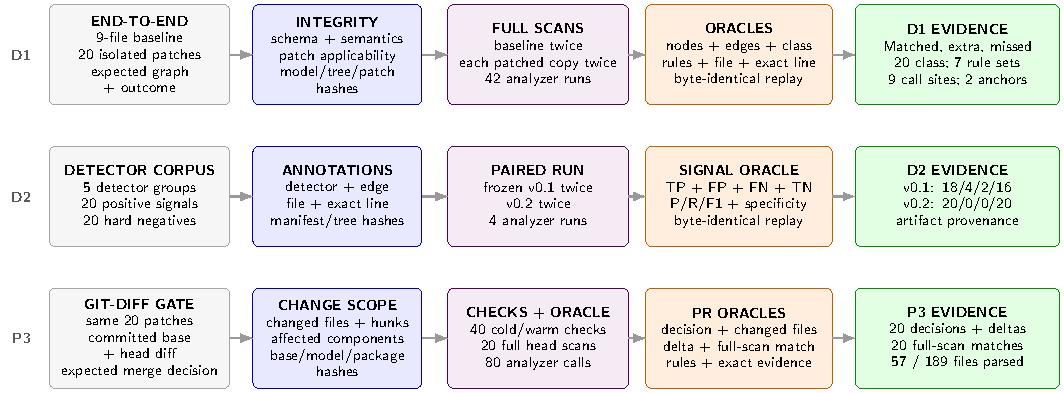
\includegraphics[width=\textwidth]{figures/Fig-2.pdf}
  \caption{Controlled verification protocol. D1 measures full-repository reconstruction and classification, D2 isolates detector signals, and P3 replays D1 as cold and warm Git-diff pull-request checks. All three routes use co-developed development data.}
  \Description{The first route validates 20 isolated executable patches and compares graphs, classifications, rules, evidence, and replay. The second validates 40 detector signals with two analyzer versions. The third commits the same baseline, applies each patch as a Git diff, performs cold and warm checks plus a full head scan, and measures decisions, changed files, architecture deltas, incremental equivalence, cache behavior, scope, evidence, and latency.}
  \label{fig:evaluation-protocol}
\end{figure*}

\subsection{Procedure}

The executed procedure for D1 was:
\begin{enumerate}
  \item validate the expected architecture, ground-truth manifest, hashes, and all patch applications;
  \item analyze the unchanged baseline twice;
  \item for each case, copy the baseline into a fresh temporary directory and apply exactly one patch;
  \item analyze the patched repository twice;
  \item compare predicted nodes, edges, classification, violated rule identifiers, and source evidence with ground truth; and
  \item remove the temporary directory before the next case.
\end{enumerate}

D1 performs 42 analyzer executions: two for the baseline and two for each of 20 cases. For D2, the manifest and annotated lines are validated before the entire repository is analyzed twice with each pinned analyzer version. Each observed relationship is expanded into detector--edge--file--line signals and compared with the annotations. D2 therefore adds four recorded executions, 46 across the reported current and historical Phase 2 evidence. The continuously rerun v0.2 gate executes 44 of them and verifies the frozen v0.1 package without rewriting that historical result.

P3 performs 40 change-scoped checks, one cold and one warm per case. Each cold check invokes a full baseline analysis and an affected-component analysis; each warm check reuses the baseline cache and invokes only the affected-component analysis. An additional full head scan per case verifies the incremental result, giving 80 analyzer calls. The normalized results compared across cold and warm runs exclude elapsed time and cache-hit state but retain changed files, affected components, graph delta, findings, evidence, and scan scope. The oracle must match head classification, decision, finding set, graph delta, and scanned-file count.

Repeated results are compared as normalized JSON. The benchmark workflow installs SHA-256-verified runtime packages and executes the Phase 2 and Phase 3 protocols plus the PASS/BLOCK/REVIEW quickstart from clean \texttt{ubuntu-latest} and \texttt{windows-latest} checkouts; both jobs passed for benchmark audit commit \texttt{5fe3679}.

\subsection{Metrics}

D1 reports counts of matched, extra, and missed graph items, with changed items separated from repeated baseline structure. For D2 only, TP and FN count annotated positive detector signals, and TN and FP count explicitly annotated hard negatives. Its descriptive precision, recall, F1, and specificity are
\begin{align}
  \operatorname{Precision} &= \frac{TP}{TP+FP},\\
  \operatorname{Recall} &= \frac{TP}{TP+FN},\\
  F_1 &= 2\cdot\frac{\operatorname{Precision}\cdot\operatorname{Recall}}
  {\operatorname{Precision}+\operatorname{Recall}},\\
  \operatorname{Specificity} &= \frac{TN}{TN+FP}.
\end{align}
We report both complete-graph and patch-changed node and edge counts. When both expected and predicted changed sets are empty, the case is an exact match but contributes no positive item to the aggregate TP/FP/FN counts. D2's TP, FP, FN, and TN units are annotated detector signals rather than distinct graph edges; several positive source locations may support the same edge.

Classification agreement is measured across all 20 cases. Rule-set agreement is measured on the seven violation cases. File and exact-line agreement are measured on the 11 finding-bearing cases; exact-line agreement means that at least one evidence item for the matched finding has the expected file and line. Determinism requires byte-identical normalized output across duplicate executions.

P3 additionally measures exact merge-decision, changed-file-set, architecture-delta, and incremental/full-scan agreement. Incremental scope is
\begin{equation}
  r_{\mathrm{parse}}=\frac{\sum_i |T_i^{\mathrm{parsed}}|}{\sum_i |T_i^{\mathrm{head}}|},
\end{equation}
where $T_i^{\mathrm{parsed}}$ contains TypeScript files parsed in affected components and $T_i^{\mathrm{head}}$ contains TypeScript files represented by the reconstructed head graph. Cache correctness requires a miss followed by a hit for every isolated case and identical normalized results. Cold and warm check latency are summarized by median and 95th percentile; no inferential comparison is made.

\subsection{Engineering Acceptance Criteria}

Before reporting the controlled run, the D1 engineering exit gate required node and edge precision and recall of at least 0.85 for both complete and changed graphs, exact classification for every case, exact violated-rule sets, matching evidence files and lines, deterministic replay, and repository-specific coverage thresholds. D2 v0.2 additionally required zero missed positive signals, zero unexpected detections, all 20 hard negatives rejected, and byte-identical replay. P3 required exact classification, decision, changed-file sets, architecture deltas, rule sets, source files and lines for all applicable cases; full-scan equivalence, cache hits, and identical normalized replay for all repeated checks; and cross-platform completion of the full benchmark workflow. The value 0.85 is an engineering prototype threshold rather than a statistically derived standard. Passing these criteria verifies the declared regression contract only; it does not establish superiority to an external tool or accuracy on unseen repositories.

\section{Controlled Verification Results}

\begin{table*}[t]
  \caption{D1 counts on 20 co-developed patches. The five changed nodes and 12 changed edges are regression items, not independent samples of general accuracy; full-graph counts repeat baseline structure.}
  \label{tab:detection-results}
  \centering
  \small
  \begin{tabular}{lrrr}
    \hline
    Measure & Matched & Extra & Missed \\
    \hline
    Full-graph nodes & 105 & 0 & 0 \\
    Full-graph edges & 108 & 0 & 0 \\
    Changed nodes & 5 & 0 & 0 \\
    Changed edges & 12 & 0 & 0 \\
    \hline
  \end{tabular}
\end{table*}

\begin{table}[t]
  \caption{Decision, evidence, and replay outcomes on controlled D1 cases.}
  \label{tab:outcome-results}
  \centering
  \small
  \begin{tabular}{lrr}
    \hline
    Measure & Matches & Total \\
    \hline
    Classification & 20 & 20 \\
    Violation rule set & 7 & 7 \\
    Evidence file & 11 & 11 \\
    Evidence exact line & 11 & 11 \\
    Deterministic cases & 20 & 20 \\
    \hline
  \end{tabular}
\end{table}

\begin{table}[t]
  \caption{P3 Git-diff gate outcomes and measured scope on the D1 replay.}
  \label{tab:phase3-results}
  \centering
  \small
  \begin{tabular}{lr}
    \hline
    Measure & Result \\
    \hline
    Classification agreement & 20/20 \\
    Merge-decision agreement & 20/20 \\
    Changed-file agreement & 20/20 \\
    Architecture-delta agreement & 20/20 \\
    Incremental/full-scan agreement & 20/20 \\
    Violation rule-set agreement & 7/7 \\
    Exact evidence line & 11/11 \\
    Cache hit on repeated check & 20/20 \\
    Normalized cold/warm replay & 20/20 \\
    Incremental files / head files & 57/189 \\
    Cold median / p95 (ms) & 518.51 / 531.05 \\
    Warm median / p95 (ms) & 242.62 / 249.30 \\
    \hline
  \end{tabular}
\end{table}

\begin{table*}[t]
  \caption{D2 within-tool regression confusion matrices for the frozen v0.1 and provenance-aware v0.2 analyzers on the same co-developed 40-signal corpus.}
  \label{tab:pattern-results}
  \centering
  \small
  \begin{tabular}{lrrrrrrrr}
    \hline
    & \multicolumn{4}{c}{v0.1} & \multicolumn{4}{c}{v0.2} \\
    Detector & TP & FP & FN & TN & TP & FP & FN & TN \\
    \hline
    \texttt{fetch} & 4 & 0 & 0 & 4 & 4 & 0 & 0 & 4 \\
    PostgreSQL & 4 & 1 & 0 & 3 & 4 & 0 & 0 & 4 \\
    Redis & 2 & 0 & 2 & 4 & 4 & 0 & 0 & 4 \\
    AMQP publish & 4 & 2 & 0 & 2 & 4 & 0 & 0 & 4 \\
    AMQP consume & 4 & 1 & 0 & 3 & 4 & 0 & 0 & 4 \\
    \hline
    Overall & 18 & 4 & 2 & 16 & 20 & 0 & 0 & 20 \\
    \hline
  \end{tabular}
\end{table*}

\textbf{RQ1: graph reconstruction and detector signals.}
The unchanged repository was reconstructed as five components and five relationships with a no-impact classification. Table~\ref{tab:detection-results} reports no false positive or false negative in D1. Full-graph totals aggregate 105 expected nodes and 108 expected edges across 20 patched repositories. Only five node changes and 12 edge changes contribute positive changed-graph items. These finite, co-developed cases test contract agreement; they do not estimate performance on unseen projects.

Table~\ref{tab:pattern-results} gives the signal-level regression result. On D2, v0.1 achieved precision 0.818, recall 0.900, F1 0.857, and specificity 0.800. Its four false positives were a PostgreSQL-shaped local query, two AMQP-publish lookalikes, and an AMQP-consume lookalike; its two false negatives were Redis \texttt{hSet} and \texttt{lPush}. On the same annotated signals, v0.2 matched all 20 positives and rejected all 20 annotated negatives (precision, recall, F1, and specificity each 1.000 on this corpus). Package-provenance tracking removed the four method-name false positives, while the expanded Redis operation set recovered the two missed positives. Because D2 was constructed from known v0.1 weaknesses, this is targeted regression evidence and not an estimate over arbitrary TypeScript syntax or an external baseline comparison.

\textbf{RQ2: change classification.}
ArchSync matched all 20 D1 labels: nine no-impact, seven violation, and four evolution cases. It also matched the complete expected rule-identifier set for all seven violations. The added allow and require-path cases exercise rule semantics beyond direct deny and require checks. Redis, AMQP, Fraud Service, and payment-cache additions were classified as evolution rather than violation, preserving a human-review path.

\textbf{RQ3: evidence localization.}
All 11 finding-bearing D1 cases contained the expected file and at least one evidence item at the exact expected line. Violation cases pointed to either the introducing call site or, for a missing required edge or path, a deterministic component anchor. Evolution cases pointed to the operation that created the new observed relationship. The metric does not evaluate uniqueness or ranking when multiple evidence items exist.

\textbf{RQ4: determinism and reproducibility.}
The D1 baseline and all 20 cases produced byte-identical normalized JSON across duplicate executions, giving 42 current-version executions with no replay mismatch. Both D2 analyzer versions were also deterministic across their duplicate runs. P3 produced identical normalized cold and warm results for 20/20 cases, matched all 20 declared architecture deltas, matched a separate full head scan in all 20 cases, and hit the baseline cache on every repeated check. As Table~\ref{tab:phase3-results} shows, component-incremental analysis parsed 57 of 189 TypeScript file instances, $r_{\mathrm{parse}}=0.3016$. On the recorded Windows environment, warm median latency was 242.62 ms compared with 518.51 ms cold, a descriptive 53.2\% reduction; warm p95 was 249.30 ms compared with 531.05 ms cold. Local verification reproduced all stored results and repository gates. GitHub Actions independently reproduced the functional benchmark, detector, and Git-diff evidence on both \texttt{ubuntu-latest} and \texttt{windows-latest}; timing values were not treated as cross-platform acceptance thresholds.

\textbf{Boundary of the reported evidence.}
The observations above come from D1, D2, and the P3 reuse of D1. No external-tool result is accepted into this evaluation, and no common label mapping has been established for comparative scoring. The internal v0.1--v0.2 detector comparison and incremental/full-scan equivalence therefore answer different questions from an external baseline: the former exposes targeted regression behavior, while the latter checks whether scoped execution preserves this implementation's full-scan result.

Exact agreement with these oracles does not establish that the expected architecture is complete or appropriate for another system. In particular, a missed relationship outside the detector vocabulary can be absent from both incremental and full scans without producing an equivalence mismatch. Similarly, duplicate executions can reproduce the same incorrect inference. The graph, evidence-location, decision, and replay checks are complementary consistency checks; they do not substitute for independently authored semantic labels or a separately evaluated tool.

\section{Discussion}

The controlled verification provides a positive feasibility result for the defined TypeScript/Node.js slice. For RQ1, deterministic AST detectors reconstructed every expected node and edge represented by D1, while D2 exposed six concrete v0.1 signal errors that the provenance-aware implementation corrected. For RQ2, the rule engine correctly gave violation precedence over topology evolution, while the REVIEW path avoided treating every new technology as forbidden. For RQ3, source locations made findings inspectable without asking a reviewer to rediscover the relevant call. For RQ4, normalized ordering and evidence deduplication removed observed replay variation, and P3 showed that the same result contract can be applied to an incrementally reconstructed Git head without diverging from a full-scan oracle on these controlled cases.

The zero-error v0.2 result must be interpreted with the denominators in Tables~\ref{tab:detection-results}--\ref{tab:pattern-results}. Nine no-impact cases contain no changed graph items. D1 contains only five changed nodes, 12 changed edges, seven violation rule sets, and 11 finding-bearing cases. D2 contains 20 positives and 20 deliberately selected hard negatives, four of each per detector. Moreover, both datasets and the analyzer were co-developed. The result is evidence that the implemented contracts and regression scenarios agree, but it is not an unbiased estimate of performance on unseen repositories.

The v0.1--v0.2 comparison illustrates why end-to-end patches alone are insufficient. Repeated baseline structure can dominate aggregate graph counts, and ordinary no-impact patches may not contain adversarial method-name collisions. Exact source-line signal annotations made false positives and false negatives visible and linked the implementation change to measured behavior. Nevertheless, because D2 was designed after observing v0.1, its value is regression protection and causal diagnosis rather than external validation. It is not a competitor baseline. An external comparison remains proposed and was not executed within the reported evaluation. A module-import analyzer and a typed service-call detector can expose different relations; a common label mapping has not yet been established. A useful comparator protocol must first define equivalent relationships or independently label a shared abstraction. Until that mapping and accepted results exist, neither comparative accuracy nor superiority is supported.

The three-way decision is practically significant even in this study. Cases that bypassed architectural rules were blocked, whereas non-forbidden Redis, AMQP, service, and cache additions were surfaced for review. P3 applies this distinction only to findings introduced at the head: a pre-existing baseline violation remains visible but does not block an unrelated patch, while a patch that removes it is recorded as resolving the finding. This supports gradual adoption without silently accepting new drift. Missing-edge evidence also exposes an inherent limitation: because an absent call has no call site, ArchSync anchors the finding to a deterministic source location in the responsible component.

The living-architecture claim is deliberately governed. The Observed Graph changes whenever source changes, but the expected graph is not inferred back into design. A REVIEW result is a proposal, not approval. The supplied CI workflow turns exit status into a merge gate and emits annotations and a report; a repository must separately protect model changes with architecture-owner review. Without that policy, the technical gate alone cannot prevent a contributor from changing both code and contract to self-approve an evolution.

P3's measured scope and latency are engineering observations, not a scalability result. Parsing 57 of 189 file instances shows that component scoping avoided parsing 69.84\% of head-file instances in this corpus. The 53.2\% median cold-to-warm reduction also includes Git process startup, diff parsing, cache I/O, conformance, and reporting. The benchmark is small, runs sequentially on one machine, and does not isolate those costs or compare against alternative incremental analyzers.

A stronger next experiment should freeze v0.3, construct a blinded holdout through independent reviewers, and evaluate multiple real TypeScript repositories and pull-request histories. It must also run a pinned external comparator on the common dependency subset and retain configuration, raw output, failures, and a capability-mapping table so unsupported relationships are not scored unfairly. Challenge cases should include wrapper libraries, re-exports, dynamic endpoint construction, dependency injection, unconventional monorepos, generated code, and runtime-only dependencies. A team pilot should measure annotation comprehension, approval delay, false-block burden, and attempts to change the model alongside implementation. The Core model and conformance engine can be reused for Java, Python, C\#, or Go, but each language requires a separately implemented analyzer and language-specific benchmark before cross-language claims are justified.

\section{Threats to Validity}

\textbf{Construct validity.}
Node, edge, classification, and evidence measures capture detectable topology and explicit rules, not component responsibility, architectural rationale, or runtime quality attributes. Exact-line agreement requires at least one matching evidence item and does not measure ranking, completeness of all supporting locations, annotation comprehension, or reviewer effort. Changed-file agreement checks Git scope, not whether the resulting report is sufficient for an architecture decision. The parsed-file fraction measures AST input scope rather than CPU work. D2 treats annotated file-line-detector-edge tuples as signals, so multiple signals may support one relationship. Its specificity covers the declared hard negatives, not all unannotated syntax.

\textbf{Internal validity.}
The authors curated the analyzer and both datasets. Although D1 topology intent was established in Phase 1, executable patches and exact evidence lines were refined during Phase 2 integration. P3 reuses those same patches and was developed against their known labels, so its complete decision agreement is a regression result, not independent validation of the Git-diff design. D2 was explicitly authored after v0.1 and used to guide v0.2, creating similar benchmark-tuning and confirmation risks. Schema checks, mutation tests, isolated patch application, source-line annotations, frozen artifacts, hash binding, and raw predictions prevent accidental inconsistency and retrospective number changes but do not provide independent ground-truth judgment.

\textbf{External validity.}
The study contains one small synthetic TypeScript/Node.js system, 20 changes, and 40 controlled detector signals. Phase 3 checks working-tree and feature-branch Git states but not a longitudinal project history, large monorepository, or human approval process. The current private repository plan did not permit required-check or ruleset enforcement, so the workflow, annotations, exit decisions, and CODEOWNERS were evaluated as technical artifacts rather than as a non-bypassable production merge policy. Detectors cover selected \texttt{fetch}, \texttt{pg}, Redis, and AMQP patterns. Results may not generalize to wrapper libraries, dynamic endpoints, reflection, dependency injection, unconventional monorepos, generated code, other languages, infrastructure-as-code, or runtime-only relationships. The architecture and conformance contracts are designed to be language-neutral, but only the TypeScript analyzer has empirical evidence.

\textbf{Comparative validity.}
No external comparison was executed within the reported evaluation, and no accepted comparator result or common label mapping is available. The v0.1--v0.2 comparison uses two ArchSync revisions on a corpus derived from known v0.1 weaknesses and therefore measures within-tool regression behavior only. Tools based on module imports can expose a different observable relation set from ArchSync's HTTP, database, cache, and messaging detectors. A future comparison must freeze a common capability subset, tool versions, configurations, dependency-resolution conditions, repositories, and independently reviewed ground truth before inspecting outputs. Until then, the paper makes no claim that ArchSync is more accurate, faster, or more useful than an existing tool.

\textbf{Literature-positioning validity.}
Related Work is a purposively scoped narrative synthesis, with source-selection and interpretation bias. Its emphasis on recent work and a small set of foundational references can omit relevant approaches, and the selection does not follow formal systematic-review inclusion/exclusion criteria or independent dual screening. Related publications may share projects, datasets, or tool implementations, so their findings are not necessarily independent. Coverage completeness and absence-of-evidence claims are outside the scope of this review design. The cited work supports design context and bounded comparisons, not exhaustive novelty or comparative-superiority claims. These are limitations of the chosen narrative method, not temporary gaps awaiting completion of another review.

\textbf{Conclusion validity.}
D1 has only five positive changed-node items, 12 positive changed-edge items, seven violation rule sets, and 11 evidence-bearing cases. D2 has 20 positive and 20 hard-negative signals. P3 has 20 cold and 20 warm checks over the same D1 changes. Zero-error agreement on these finite, co-developed sets is a feasibility and regression result, not a statistical claim about a population. Latency percentiles are descriptive measurements from one environment; no confidence interval or significance test is used because the samples are neither independent random draws nor a defined workload population.

\textbf{Reliability.}
Dependencies and inputs are pinned and hashed, paths and JSON are normalized, patches are isolated, and every current input is executed twice. Phase 3 commits the same baseline metadata for each case, requires a cache miss followed by a hit, compares the incremental head with a separate full scan, and excludes timing and cache state from normalized replay comparison. Raw timing samples are retained and their medians and percentiles are recomputed by the verifier. Local Windows verification reproduced the result with Node.js 22.16.0 and the repository-declared pnpm 11.16.0 toolchain. GitHub Actions additionally reproduced the functional gate on clean \texttt{ubuntu-latest} and \texttt{windows-latest} runners using SHA-256-verified artifacts. The v0.1 challenge result is frozen and provenance-validated rather than re-executed by the current gate. Timing is retained only for the recorded Windows environment. These controls reduce, but do not eliminate, platform and toolchain threats.

\section{Conclusion and Future Work}

ArchSync implements a deterministic bridge between a declared architecture contract and a source-derived TypeScript service graph. On the co-developed development datasets, its graph, classification, evidence-location, replay, and incremental/full-scan outputs agree with the declared regression oracles. The targeted detector corpus also exposes concrete errors in the earlier analyzer and verifies that provenance tracking addresses those cases.

These findings show that the current contracts, detectors, and Git-diff workflow operate coherently on their controlled scope. They do not establish general accuracy, comparative advantage, or governance effectiveness because the datasets are synthetic and co-evolved with the implementation, an external comparison remains proposed without accepted results or a common label mapping, and no independent real-world holdout exists. ArchSync keeps design changes human-governed: the analyzer never rewrites the approved model, violations block, and evolution requires review. The immediate research priorities are an independently curated multi-repository holdout, a capability-matched comparison with an existing TypeScript dependency-conformance tool, and a real pull-request pilot. Only after those gates produce auditable evidence should the paper make claims about external accuracy, performance, or developer value.

\makeatletter
\if@ACM@anonymous\else
\noindent\begin{minipage}{\columnwidth}
\section*{Author Information and Contributions}

\noindent\textbf{Vo Duc Hieu} (ORCID: \href{https://orcid.org/0009-0007-5389-5177}{0009-0007-5389-5177}) - Conceptualization; Methodology; Software; Project administration; Writing.

\noindent\textbf{Tran Minh Hoang} (ORCID: \href{https://orcid.org/0009-0000-0302-1841}{0009-0000-0302-1841}) - Software; AI methodology; Validation.

\noindent\textbf{Ha Hoang Bach} (ORCID: \href{https://orcid.org/0009-0000-5118-0660}{0009-0000-5118-0660}) - Investigation; Data curation; Formal analysis; Evaluation.

\noindent\textbf{Le Van Kiet} (ORCID: \href{https://orcid.org/0009-0007-8434-882X}{0009-0007-8434-882X}) - Software; Validation; Reproducibility.
\end{minipage}
\fi
\makeatother


\bibliographystyle{ACM-Reference-Format}
\bibliography{references}

\end{document}
